% Homework #3
% COSC552 HCI
%
% Byron Heads
% E00062946

\documentclass[12pt]{article}

\usepackage{graphics}
\usepackage{hyperref}

\title{Homework Set 3 \\
    COSC552 HCI}
\author{ Byron Heads \\
    E00062946 }
\date{\today}

\begin{document}
\maketitle

\section*{A}
\resizebox{\columnwidth}{!}{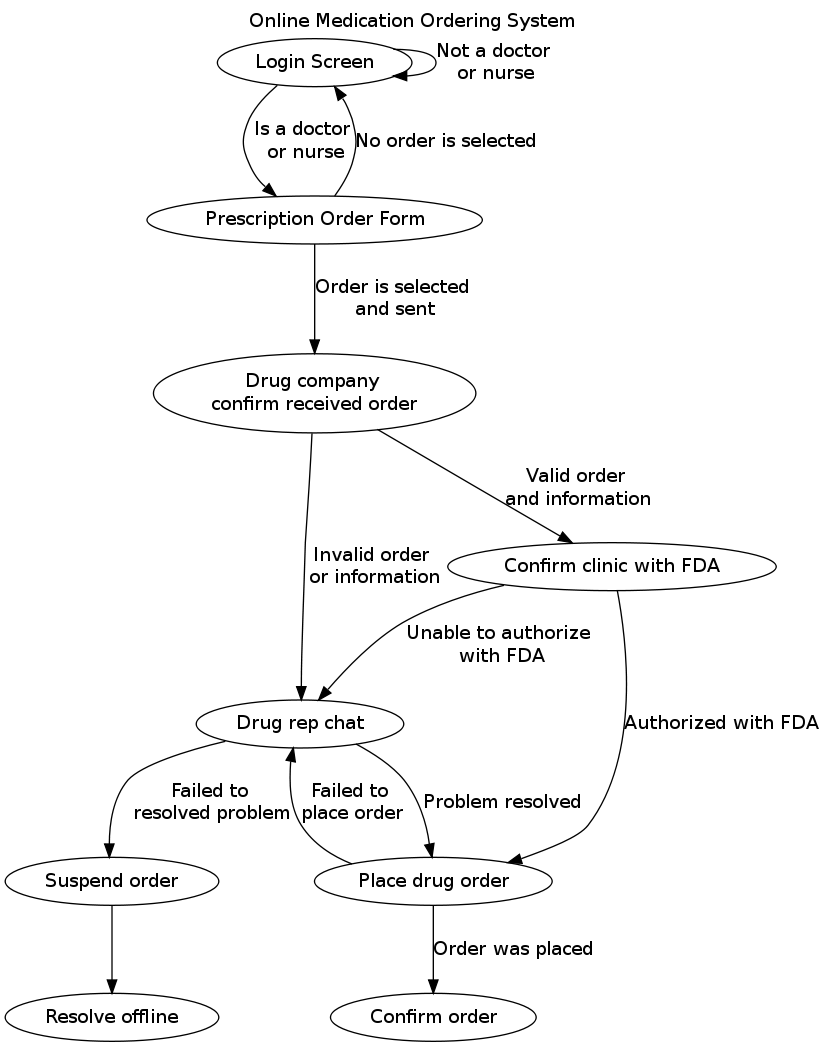
\includegraphics{hw3.png}}

\section*{B}

Training new doctors and nurses on the system can be done through a series of collaborative technologies.  One method is to develop a training mode, this is similar to demos or tutorials found in video games.  The training mode runs the user step by step through the process of placing fake orders.  The training mode controls the flow of the learning process.  This would include having the user make mistakes and how they can fix them.  The training mode asks the user questions during and after the training scenarios.  The user is allowed to email or ask other staff members for help with the questions.  These test can give the user an idea how much of the process they understand.

Other technologies such as instant messaging can be deployed to allow staff members to communicate with each other.  They can use it to ask questions and give answers to coworkers.  Free services such as Google Talk (\url{http://google.com/talk}) can be used with open source software like Pidgin (\url{http://pidgin.im}) to create an encrypted communication between two or more staff members.  This technology can be used for free and with encryption is secure allowing sensitive information to be sent.  This technology can also be used for video chatting between staff members.  Video conferencing is a useful technology in collaboration.

Other tools such as TightVNC (\url{http://www.tightvnc.com}) can be used to allow another staff member take control over another computer.  This can be used to allow another staff member walk a coworker through the process of using the interface and placing an order.  This software is available for free, there are other commercial version of this software as well.

The software in these examples were chosen because they are FOSS ( Free and Open Source Software ).  These programs can be downloaded and used for free by the clinic.  These programs used by many users and is know to be stable.  They are able to run on all modern operating systems and are maintained by programmers who use these programs.  Bugs and security updates are release as fast as the problems are discovered.  Commercial software can be used in place, but they often have limitations, such as which operating system they can be run on and which software it can work with. 

\end{document}

